\documentclass[a4paper,utf8]{article}
\usepackage[heading,fancyhdr]{ctex}
\usepackage{amsmath,amssymb,geometry,lastpage,ulem}
\usepackage{array,tabularx}
\usepackage{siunitx}
\usepackage{graphicx}
\lineskiplimit=1pt
\lineskip=3pt
\geometry{
    top=25.4mm, 
    left=25mm, 
    right=25mm, 
    bottom=25mm,
    headsep=5.9mm,
}
\ctexset{
    section = {format+=\raggedright}
}
\newcommand{\fgref}[1]{图~\ref{#1} }
\newcommand{\seqref}[1]{式~(\ref{#1})}
\pagestyle{fancy}
\fancyhf{} \fancyhead[C]{材料科学基础实验} \fancyfoot[C]{\thepage\;/\;\pageref{LastPage}}
\begin{document}
\begin{center}
    {\mbox{}\\[7em]\zihao{2}\bfseries\songti%
    材料科学基础实验预习报告}\\[34mm]
    {\zihao{-3}\bfseries\songti
    实验名称:\uline{\hfill\mbox{绝缘材料的相对介电常数和介质损耗因数测试}\hfill} \\[2.9mm]
    学\quad 号:\uline{\makebox[25mm]{22301077}}\hfill
    姓\quad 名:\uline{\makebox[25mm]{张蕴东}}\hfill
    班\quad 级:\uline{\makebox[25mm]{22高分子}} \\[2.9mm]
    合作者:\uline{\makebox[25mm]{}}\enspace~
    桌\quad 号:\uline{\makebox[25mm]{}}\hfill\mbox{}\\[2.9mm]
    指导教师:\uline{\makebox[30mm]{艾斌}}\hfill\mbox{} \\[2.9mm]
    实验日期:\uline{\makebox[30mm]{}}\hfill\mbox{} \\[58.7mm]
    }
\end{center}
\newpage
\section{实验目的}
    \begin{itemize}
        \item 了解 Q 表法和变电纳法测量绝缘材料相对介电常数和介质损耗因数的原理
        \item 学会用 Q 表法和变电纳法测量绝缘材料的相对介电常数和介质损耗因数
        \item 了解影响测量结果准确性的因素及避免方法
    \end{itemize}
\section{实验原理}%简单描述,含必要的公式和附图;
    \subsection{基本概念}
        \subsubsection{相对介电常数和绝对介电常数}
            当电容器的两个极板之间充以绝缘材料时,其电容 $C_x$ 与两个极板之间充以真空时的电容 $C_0$ 之比就定义为该绝缘材料的相对介电常数 $\varepsilon_r$,用公式可表示为:
            \begin{equation}
                \varepsilon_r = \frac{C_x}{C_0}
            \end{equation}
            在标准大气压下,干燥空气的相对介电常数为 1.00053 ,因此,人们在实际测量绝缘材料的相对介电常数时,常常使用两极板充以空气时的电容 $C_a$ 来代替 $C_0$,这种替代所引入的误差常常是可以忽略的。\par
            绝缘材料的介电常数(或绝对介电常数)$\varepsilon$ 定义为该材料的相对介电常数$\varepsilon_r$ 与真空介电常数 $\varepsilon_0$ 的乘积。在 SI 中,真空介电常数$\varepsilon_0$为:
            \begin{equation}
                \varepsilon_0=\SI{8.854d-12}{\farad\per\metre}\approx \frac{1}{36\pi}\times\SI{e-9}{\farad\per\metre}\label{eq2}
            \end{equation}
            如果不考虑边缘效应,以相对介电常数为$\varepsilon_r$的绝缘材料为介质的平行板电容器的电容为:
            \begin{equation}
                C_x=\frac{\varepsilon_0 \varepsilon_r S}{d}\label{eq3}
            \end{equation}
            式中 $S$ 和 $d$ 分别为平行板电容器的极板面积和间距,各物理量的单位均使用国际单位制。将\seqref{eq2}代入\seqref{eq3}式可得:
            \begin{equation}
                C_{x}=\frac{\varepsilon_{r} S}{36 \pi d} \times 10^{-9} ~\unit{\farad}=\frac{\varepsilon_{r} S}{36 \pi d} ~\unit{\nano\farad}=\frac{100 \varepsilon_{r} S}{3.6 \pi d} ~\unit{\pico\farad}\label{eq4}
            \end{equation}
            由\seqref{eq4}式可得:
            \begin{equation}
                \varepsilon_r=\frac{3.6 \pi d C_x}{100 S}
            \end{equation}
            式中,电容$C_x$以 $\unit{\pico\farad}$ 为单位,电容器的极板面积 $S$ 和间距 $d$ 分别以 $\unit{\metre\squared}$ 和 $m$ 为单位。\par 
            如果平板电极为圆形,且其直径为 $D_0$ 时,相对介电常数的表达式可进一步写作:
            \begin{equation}
                \varepsilon_r=\frac{3.6\pi dC_x}{100S}=\frac{14.4dC_x}{100D_0^2}
            \end{equation}
            式中,极板直径 $D$ 和间距 $d$ 均以 $\unit{\metre\squared}$ 为单位,电容$C_x$以 $\unit{\pico\farad}$ 为单位。
        \subsubsection{介质损耗角和介质损耗因数}
            在交流电路中,由于理想电容的电流始终超前电压 90°相位,所以理想电容在充放电过程中不会消耗能量。作为对比,由绝缘材料作为介质的实际电容器在充放电过程中会消耗能量,其原因是电介质内部的电荷在外加交变电场的作用下被反复极化,电荷的频繁极化运动(取向极化或位移极化)需克服材料内部的摩擦力做功,另一方面,还有一部分能量以漏电电流产生焦耳热的形式消耗。这两种能量消耗都以热能的形式释放并造成电容器温度升高。\par 
            如果把一块圆柱状薄片电介质的两个底面镀上电极,则它构成了一个平行板电容器,可以用一个理想电容和一个电阻的并联来描述它在交流电路中的性能,如图 1 所示,介质损耗角$\delta$ 被定义为由电介质材料组成的实际电容器上的电压 U 与电流 I 之间的相位角$\varphi$ 的余角$\delta$ ,即$\delta  = 90\deg - \varphi$ ,而介质损耗因数 D 被定义为介质损耗角$\delta$ 的正切值,即
            \begin{equation}
                D=\tan\delta=\frac{1}{\omega C_{p}R_{p}}\label{eq7}
            \end{equation}
            之所以使用介质损耗因数 $D$ 来描述电介质消耗的功率,原因在于:如果我们以角频率为$\omega$ 、有效值为 $U$ 的正弦交流电加在电容 $C_p$ 和电阻 $R_p$ 组成的并联电路的两端,消耗在电阻上的功率可表示为 $P = UIR = UIC\tan{\delta } = U^2 \omega C_p \tan{\delta }$。由上式可知,在电源电压、角频率和电容 $C_p$一定的前提下,消耗在电阻 $R_p$ 上的功率与介质损耗因数 $D$ 成正比。
            \begin{figure}[!ht]\centering
                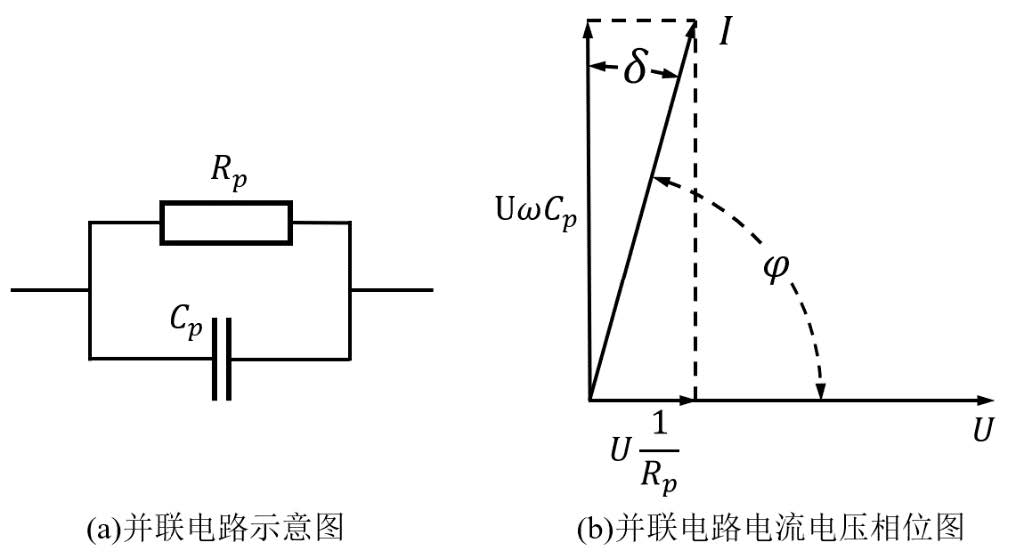
\includegraphics[width=100mm]{fg1.jpg}\
                \caption{有损耗的电容器的并联等效电路图及相应的电流和电压相位图\label{fig:1}}
            \end{figure}
        \subsubsection{描述有损耗的电容器的两种等效电路}
            除了可以用\fgref{fig:1}所示的并联电路来表示一个有损耗的电容器之外,还可以用电容 $C_s$ 和电阻 $R_s$ 组成的串联电路来表示它,如\fgref{fig:2} 所示,在串联等效电路中,介质损耗因数 $D$ 可以表示为
            \begin{equation}
                D=\tan \delta=\omega C_s R_s
            \end{equation}
            由于并联电路和串联电路对同一个有损耗的电容器的表示是等价的,因此,它们应具有相同的阻抗和介质损耗因数,即
            \begin{equation*}
                    \left\{ \begin{aligned}
                        R_s+\frac{1}{j\omega C_s}&=\frac{1}{\frac{1}{R_p}+j\omega C_p}=\frac{R_p}{1+j\omega R_pC_p}=\frac{R_p-j\omega R_p^2C_p}{1+\omega^2R_p^2C_p^2}\\
                        D&=\tan\delta=\omega C_sR_s=\frac{1}{\omega C_pR_p}
                    \end{aligned} \right.
            \end{equation*}
            解得
            \begin{align}
                C_p&=\frac{C_s}{1+\tan^2 \delta}\label{eq9}\\[.5em]
                R_p&=\left( 1+\frac{1}{\tan^2 \delta} \right) R_s\label{eq10}
            \end{align}
            \seqref{eq9}和\seqref{eq10}给出了两种等效电路中串联元件参数$(C_s,R_s)$和并联元件参数$(C_s,R_s)$须满足的关系。
            \begin{figure}[!ht]\centering
                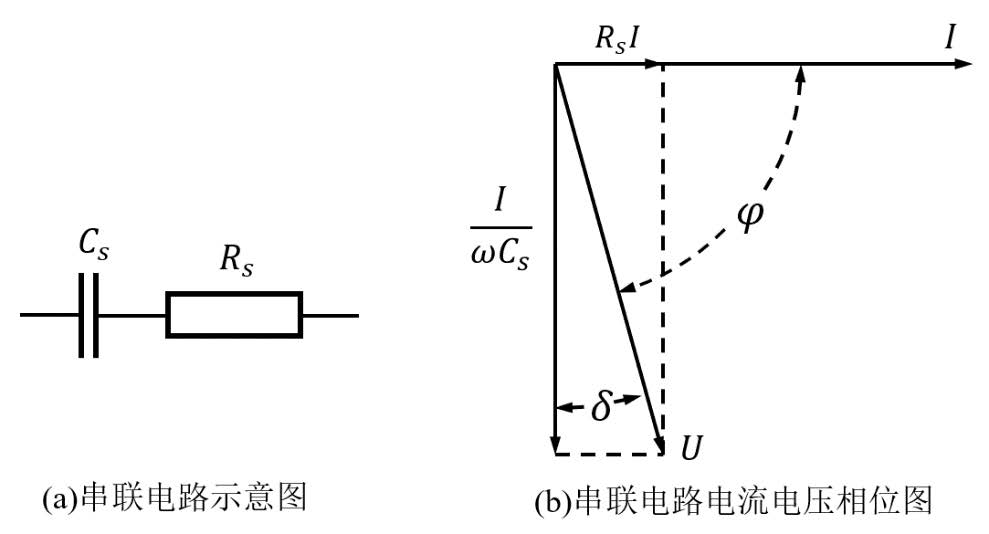
\includegraphics[width=100mm]{fg2.jpg}\
                \caption{有损耗的电容器的并联等效电路图及相应的电流和电压相位图\label{fig:2}}
            \end{figure}
        \subsubsection{品质因子 $Q$}
            品质因子 $Q$ :表示储能器件(电容或者电感)在谐振电路中每一个周期所储存的能量与每一个周期因介质损耗损失的能量之比,它在数值上等于介质损耗因数($\tan\delta$)的倒数,即
            \begin{equation}
                Q=\frac{1}{\tan\delta}\label{eq11}
            \end{equation}
        \subsubsection{复相对介电常数}
        在交变电场的作用下,电介质的相对介电常数为复数,它被称为复相对介电常数。复相对介电常数$\varepsilon^*$定义为:
        \begin{equation}
            \varepsilon^*=\varepsilon^{\prime}-j\varepsilon^{\prime\prime}=\varepsilon_r-j\varepsilon_r\tan\delta 
        \end{equation}
        由上式可知,复相对介电常数的实部就是我们通常所指的相对介电常数$\varepsilon_r$,而复相对介电常数的虚部 $\varepsilon^{\prime\prime}$表示介质损耗,它在数值上等于该绝缘材料的相对介电常数$\varepsilon_r$与介质损耗因数$\tan\delta$的乘积。
    \subsection{测试方法及原理}
        介质损耗是指电介质材料在外电场作用下因发热而引起的功率损耗。在直流电场作用下,电介质的损耗主要是由电导电流造成的电导损耗。在交流电场作用下,电介质的损耗除了电导电流造成的电导损耗以外,还有极化损耗。由于电场频繁转向,电介质的极化损耗要比电导损耗大得多,有时甚至大几千倍,因此,在某种意义上说,介质损耗通常是指交流损耗。在实际应用中,介质损耗不但会消耗电能,使元件发热影响其正常工作,而且还可能因介质损耗过大造成元件热击穿而失效。因此,介质损耗是应用于交流电场特别是高频电场中的电介质材料的一个重要品质指标,对其进行测试具有重要的意义。\par
        根据电介质材料应用领域(频率域)的不同,测量电介质材料相对介电常数和介质损耗因数的方法可分为:电桥法(小于 \unit{\mega\hertz}),谐振法(在 \unit{\mega\hertz}\~{}100 \unit{\mega\hertz}),同轴探针法\linebreak(\unit{\mega\hertz}\~{} \unit{\giga\hertz}),传输线法(\unit{\mega\hertz}\~{}100 \unit{\giga\hertz}),自由空间法(\unit{\giga\hertz}\~{}100 \unit{\giga\hertz})等。\par
        本实验利用 WY2851 Q 表、WY915 介质损耗测试装置(测试架)和标准电感组成的实验装置测量电介质材料的相对介电常数和介质损耗因数。\fgref{fig:3}(左图)给出了整个实验装置的实物照片,\fgref{fig:3}(右图)给出了测试架的实物照片。该实验装置可提供两种方法(Q 表法和变电纳法)测量材料的相对介电常数和介质损耗因数。
        \begin{figure}[!ht]
            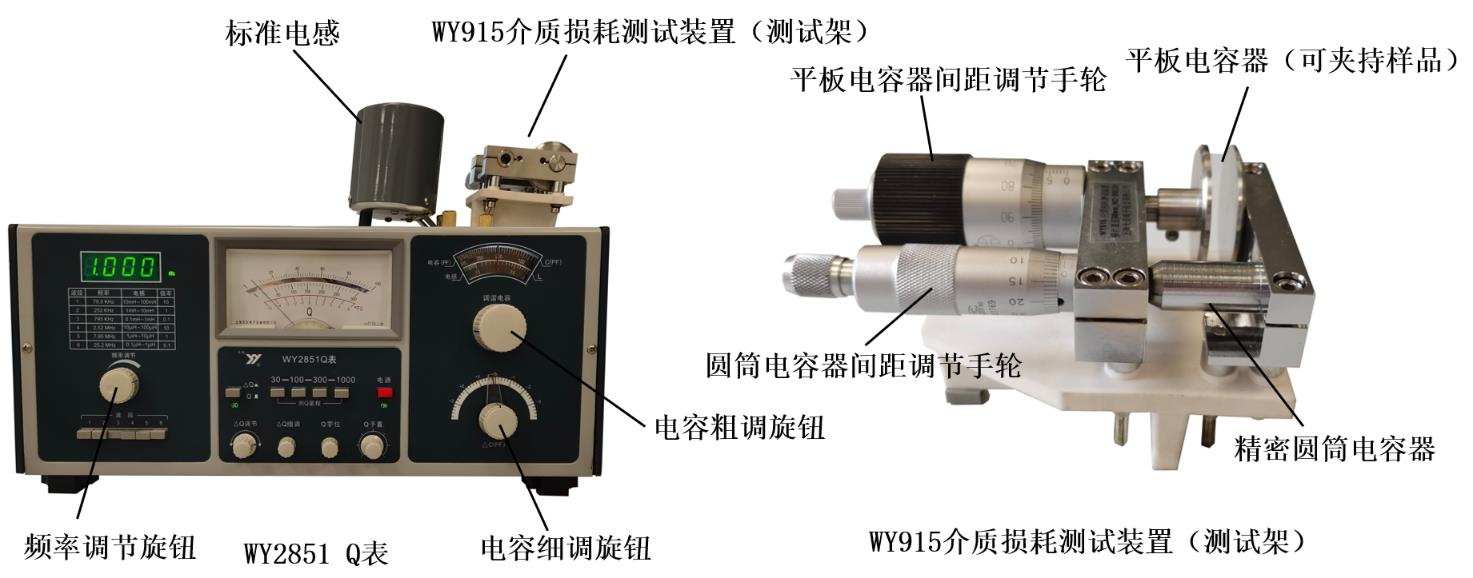
\includegraphics[width=\textwidth]{fg3.jpg}\
            \caption{整个实验装置的实物照片(左图)和测试架的实物照片(右图)\label{fig:3}}
        \end{figure}
        \subsubsection{Q 表法(谐振法)测量绝缘材料相对介电常数和介质损耗因数的原理}
            WY2851 Q 表由一个频率可调的信号发生器、可变电容 C 和连接在电容器两端的电压表 V组成。当接入标准电感 L 时,就形成了 LC 串联振荡电路,LC 串联电路中的介质损耗使用与可变电容并联的电导$G_0$表示(注:$G_0=\frac{1}{R_0}$),如\fgref{fig:4} 所示。当该 RLC 电路谐振时,电路的品质因子 Q 等于谐振时感抗($\omega L$)或容抗($\frac{1}{\omega C}$)与电阻($\frac{1}{G_0}$)之比,即 $Q = \omega L G_0 =\frac{G_0}{\omega C}$,且 L 和 C 上的电压的绝对值都等于电源电压 $U_0$ 的 $Q$ 倍,即 $Q = \frac{1}{R_0}$。由于 L 和 C 上的电压方向正好相反,两者的和为零。因为电路谐振时回路的品质因子 $Q$ 等于电压表测得的电容器两端的电压 $U_c$ 与电源(信号发生器)电压 $U_0$ 的比值,所以当信号发生器输出的电压 $U_0$ 保持恒定时,电压表上的读数$U_c$可以用谐振回路的品质因子 Q 来标定,这样就能直接从电压表上读出谐振回路的品质因子 Q,这就是 Q 表的工作原理。\par
            \fgref{fig:4}给出了谐振法(Q 表法)测量电介质材料相对介电常数和介质损耗因数的原理简图。如图所示,该测试线路由电源(信号发生器)$U_0$、标准电感 L、可变电容 C、测试线路总有效电导(不含样品)$G_0$、电压表 V、电键 S 和电介质样品的电容 $C_x$ 和电导 $G_x$ 组成。当电键 S 闭合时,意味着夹持了电介质样品的 WY915 测试架接入了 WY2851 Q 表,形成了完整的测量电介质样品相对介电常数和介质损耗因数的电路。
            \begin{figure}[!ht]\centering
                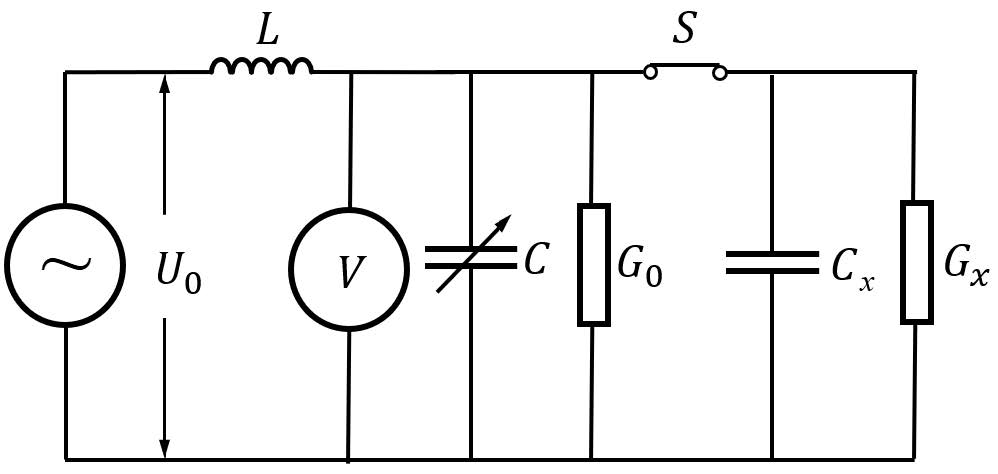
\includegraphics[width=100mm]{fg4.jpg}\
                \caption{谐振法(Q 表法)测量电介质材料相对介电常数和介质损耗因数的原理简图\label{fig:4}}
            \end{figure}\par
            谐振法测试分为两步:
            \begin{enumerate}
                \item 将 Q 表上的信号发生器的频率调到指定频率,在 Q 表的电感接线端接入电感值适当的标准
                电感,在 Q 表的电容接线端接入夹持有电介质样品的 WY915 测试架。假设夹持了电介质样品
                的平行板电容器的电容为 $C_x$,代表电介质样品介质损耗的并联电导为 $G_x$。调节 Q 表上的可变电容 $C$ 到 $C_1$ 使电路谐振,此时,Q 表的读数为 $Q_1$,根据\seqref{eq7}和\seqref{eq11},我们有(参见\fgref{fig:1}和\fgref{fig:4})
                \begin{align}
                    \frac{1}{Q_1}=\tan\delta_1&=\frac{G_0+G_x}{\omega (C_x+C_1)}\label{eq13}\\
                    \text{而且}\enskip\omega L&=\frac{1}{\omega (C_x+C_1)}\label{eq14}
                \end{align}
                式中,$G_0 + G_x$表示在 LC 串联谐振电路中接入电介质样品后电路中总的有效电导。
                \item 松开平行板电容器两极板,取出电介质样品。调节平行板电容器两极板的间距使之与样品厚度 $d$ 相同。假设极板间距等于样品厚度 $d$ 并且以空气作为介质的平行板电容器的电容为 $C_p$ 。调节 Q 表上的可变电容 $C$ 到 $C_2$ 使电路重新谐振,此时,我们有
                \begin{align}
                    \frac{1}{Q_2}=\tan\delta_2&=\frac{G_0}{\omega (C_p+C_2)}\label{eq15}\\
                    \text{而且}\enskip\omega L&=\frac{1}{\omega (C_p+C_2)}\label{eq16}
                \end{align}
                由\seqref{eq14}和\seqref{eq16}可得
                \begin{equation}
                    C_x+C_1=C_p+C_2 \Rightarrow C_x=C_p+(C_2-C_1)\label{eq17}
                \end{equation}\par
                根据电介质材料相对介电常数的定义,我们有
                \begin{equation}
                    \varepsilon_r=\frac{c_x}{c_p}=\frac{(C_2-C_1)+C_p}{c_p}\label{eq18}
                \end{equation}
                \begin{equation}
                    C_p=\frac{100\varepsilon_aS}{3.6\pi d}\:\unit{\pico\farad}=\frac{100\times1.00053\times\pi r^2\times10^{-4}}{3.6\pi d\times10^{-2}}\:\unit{\pico\farad}\approx\frac{r^2}{3.6d}\:\unit{\pico\farad}\label{eq19}
                \end{equation}
                需要说明的是,这里的$C_p$通常也被称为结构电容。由上式可知,它仅与样品厚度 $d$ 和极板半径 $r$ 有关。对于本实验,WY915 测试架上的平行板电容器的极板半径为 1.9 \unit{\centi\metre} 。至此,可利用\seqref{eq18}和\seqref{eq19}计算电介质样品的相对介电常数。
                由图 4 可知,在 Q 表中接入夹持有电介质样品的 WY915 测试架,相当于给 LC 电路接入了一个由电容 $C_x$ 和电导 $G_x$ 组成的并联支路。利用\seqref{eq7},电介质样品的介质损耗因数可表示为:
                \begin{equation}
                    \tan\delta_x=\frac{G_x}{\omega C_x}\label{eq20}
                \end{equation}
                由\seqref{eq14}和\seqref{eq16},我们有 $\omega(C_{x}+C_{1})=\omega(C_{p}+C_{2})$,$\eqref{eq13}-\eqref{eq15}$ 可得
                \begin{equation}
                    \frac{1}{Q_{1}}-\frac{1}{Q_{2}}=\frac{G_{0}+G_{x}}{\omega(C_{x}+C_{1})}-\frac{G_{0}}{\omega(C_{p}+C_{2})}=\frac{G_{x}}{\omega(C_{p}+C_{2})}\label{eq21}
                \end{equation}
                将\seqref{eq21}代入\seqref{eq20},我们有:
                \begin{equation}
                    \mathrm{tan}\delta_{x}=\frac{G_{x}}{\omega C_{x}}=\frac{C_{p}+C_{2}}{C_{x}}\biggl(\frac{1}{Q_{1}}-\frac{1}{Q_{2}}\biggr)=\frac{C_{p}+C_{2}}{C_{p}+C_{2}-C_{1}}\biggl(\frac{1}{Q_{1}}-\frac{1}{Q_{2}}\biggr)\label{eq22}
                \end{equation}
                至此,可利用\seqref{eq22}计算电介质样品的介质损耗因数。对于 Q 表法测量绝缘材料相对介电常数和介质损耗因数所涉及的公式,附录 A 给出了更详细的推导过程。
            \end{enumerate}
        \subsubsection{变电纳法测量绝缘材料相对介电常数和介质损耗因数的原理}
            WY915 测试架除了配备有平行板电容器之外,还配备了一个电容线性变化率为 \SI{0.33}{\pico\farad/\milli\metre}、长度调节范围为 0—25 \unit{\milli\metre}、分辨率为 \SI{0.0033}{\pico\farad} 的圆筒电容器,如 \fgref{fig:3} 所示。该圆筒电容器为我们提供了另外一种测量电介质材料相对介电常数和介质损耗因数的方法(变电纳法)。与谐振法相比,变电纳法通常具有更高的测量精度。\par
            变电纳法的测试方法如下:
            \begin{enumerate}
                \item 将 Q 表调到指定频率,将电感值适当的标准电感接入 Q 表,将 WY915 测试架接入 Q 表;将样品插入到 WY915 测试架上的平行板电容器中,并调节螺旋测微器使极板夹紧样品,同时记录螺旋测微器测得的样品厚度 $D_2$。调节圆筒电容器的螺旋测微器到中央位置附近(譬如 12 \unit{\milli\metre} 处)。调节 Q 表上的调谐电容使电路谐振,读取 $Q_s$ 值(其对应的电压为 $U_{rs}$);调节测试架上圆筒电容器的螺旋测微器使电路偏离谐振点(此时 Q 表起电压表的作用),使电压值降到$\dfrac{U_{rs}}{\sqrt{2}}$,而对应于同一个电压值($\dfrac{U_{rs}}{\sqrt{2}}$)有两个电容值,且位于最大谐振点 $Q_s$ 对应的电容值 $C_r$ 的两端,如\fgref{fig:5}所示,由此可确定出与 $\dfrac{U_{rs}}{\sqrt{2}}$ 对应的两个电容的差值 $\varDelta  C_s$。
                \item 调节圆筒电容器的螺旋测微器使刻度重新回到 \SI{12}{\milli\metre} 处,此时电路再次谐振。调节平行板电容器螺旋测微器松开两极板,取出电介质样品,此时电路再次偏离谐振。调节平行板电容器的螺旋测微器改变空气隙的宽度,使电路再次谐振,读取 $Q_a$ 值(其对应的电压为 $U_{ra}$),并记录螺旋测微器测得的空气隙的宽度$D_4$。调节测试架上圆筒电容器的螺旋测微器使电路偏离谐振点(此时 $Q$ 表起电压表的作用),使电压值降到 $\dfrac{U_{ra}}{\sqrt{2}}$,而对应于同一个电压值($\dfrac{U_{ra}}{\sqrt{2}}$)有两个电容值,且位于最大谐振点$ Q_a $对应的电容值 $C_r$ 的两端,如\fgref{fig:5}所示,由此可确定出与 $\dfrac{U_{ra}}{\sqrt{2}}$ 对应的两个电容的差值 $\varDelta C_a$。\par
                根据以上测量结果,可利用下面的公式计算被测样品的相对介电常数和介质损耗因数:
                \begin{align}
                    \varepsilon_r&=\frac{D_2}{D_4}\label{eq23}\\
                    \tan\delta&=\frac{\Delta C_{s}-\Delta C_{a}}{2C_{x}}=\frac{D_{4}(\Delta C_{s}-\Delta C_{a})}{2D_{2}C_{p}}=\frac{D_{4}K(M_{1}-M_{2})}{2D_{2}C_{p}}\label{eq24}
                \end{align}
                式中,$K$ 为圆筒电容器的线性变化率,其值为 \SI{.33}{\pico\farad/\milli\metre}。$M_1$ 和 $M_2$ 是圆筒电容器螺旋测微器测得的极板间距的改变量,分别对应于 $\varDelta C_s$ 和 $\varDelta C_a$ 的电容变化量。$C_p$ 是结构电容,其计算公式由\seqref{eq19}给出。对于变电纳法测量绝缘材料相对介电常数和介质损耗因数所涉及的公式,附录 B 给出了详细的推导过程。

            \end{enumerate}

            \begin{figure}[!ht]\centering
                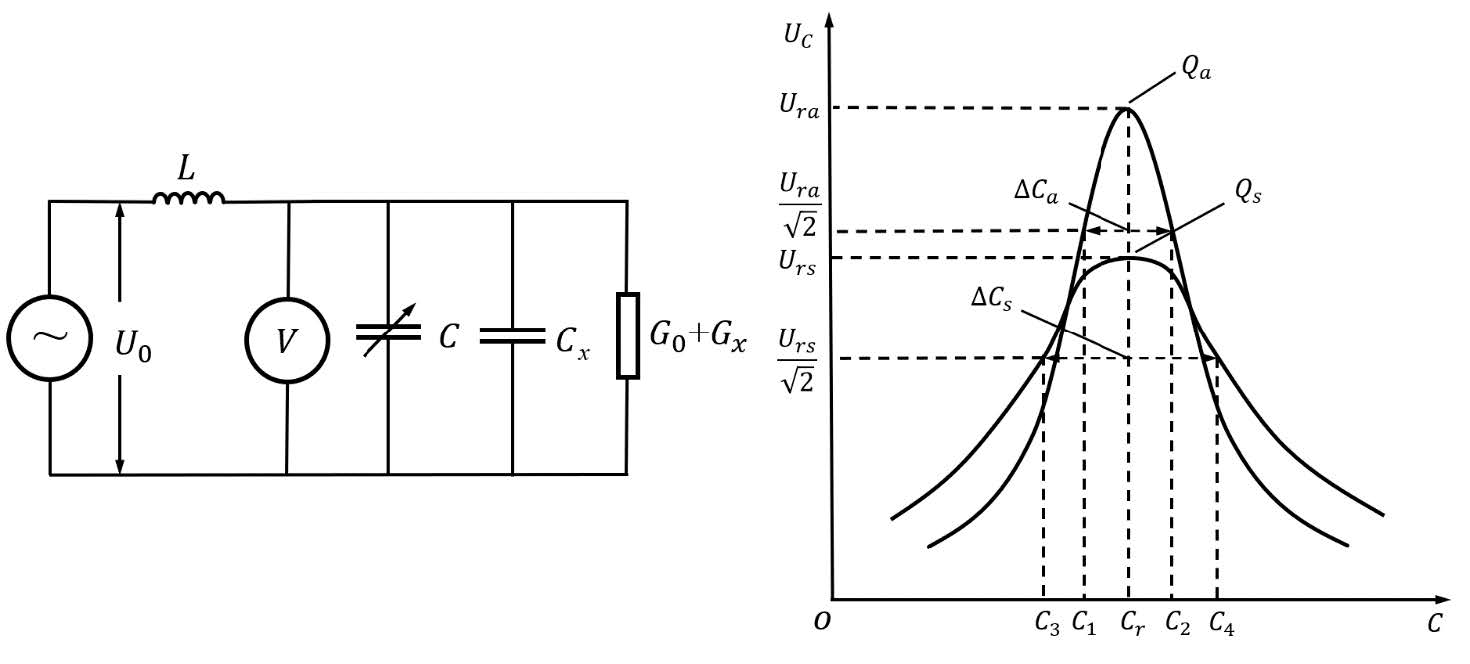
\includegraphics[width=100mm]{fg5.jpg}\
                \caption{变电纳法测量绝缘材料相对介电常数和介质损耗因数的电路图(左)和原理图(右)\label{fig:5}}
            \end{figure}

\section{实验仪器}%规格及参数
    WY2851 Q 表,WY915 介质损耗因数测试架,\SI{1}{\micro\henry} 标准电感,\SI{100}{\micro\henry} 标准电感,被测样品(印刷电路板、聚四氟乙烯和石英玻璃)。

\section{实验过程}%简述主要过程和实验内容
    \subsection{利用谐振法(或 Q 表法)测量 \SI{1}{\mega\hertz} 下三种样品(印刷电路板、聚四氟乙烯和石英玻璃)的相对介电常数和介质损耗因数}
    \begin{enumerate}
        \item 在 Q 表没有接入标准电感和电容的状态下,检查 Q 表的指针是否指零。如果不为零,应调节 Q 使 Q 表的指针指向零点。
        \item 检查 Q 表是否正常,具体做法是将频率调至 \SI{1}{\mega\hertz};将 30-100-300 三个量程按钮全部按下。将 \SI{1}{\micro\henry} 的标准电感接入到 Q 表的电感接线端(即 $L_x$)上;将微调谐电容置于 \SI{0}{\pico\farad} 处,调节主调谐电容使电路谐振,此时 Q 值应该在 190 左右,调谐电容的值在 \SI{249}{\pico\farad} 左右。如果调节主调谐电容,电路确实发生谐振且示数相仿,则说明 Q 表工作正常。
        \item 检查 WY915 介质损耗测试装置(测试架)上的平行板电容器的螺旋测微器的零点。具体做法是调节平行板电容器的螺旋测微器,使两极板接触,这时螺旋测微器的读数应该为 \SI{0}{\milli\metre}。如果螺旋测微器的读数不为 \SI{0}{\milli\metre},读取两极板接触时的刻度值记为 $D_0$(注意:调节螺旋测微器时,一定要转动调节手轮,不能直接转动测微杆,以免损坏螺旋测微器的精密螺纹,听到调节手轮发出“吱吱”的声音即可)
        \item 将 WY915 测试架接入 Q 表的电容接线端(即 $C_x$)。调节螺旋测微器手轮松开 WY915 测试架上的平行板电容器两极板,将样品插入两极板,调节测微器手轮直到两极板夹紧样品,读取刻度值记为 $D_1$,则样品厚度为 $d = D_1 - D_0$。把圆筒电容器螺旋测微器置于 \SI{12}{\milli\metre} 处(圆筒电容器螺旋测微器的调节范围为 0—25 \unit{\milli\metre})。检查 Q 表频率是否为 \SI{1}{\mega\hertz},如果不是,将 Q 表频率调节到 \SI{1}{\mega\hertz}。调节 Q 表主调谐电容使电路谐振,进一步调节 Q 表微调谐电容使 Q 表指针指到最大,记下此时的 $Q_1$ 值。与此同时,记下主调谐电容和微调谐电容之和,记为 $C_1$。
        \item 调节螺旋测微器手轮,松开 WY915 测试架上的平行板电容器的两极板,取出样品。重新将两极板间距调到样品厚度处,即平行板电容器螺旋测微器处于刻度 $D_1$ 处。圆筒电容器螺旋测微器处于 \SI{12}{\milli\metre} 处不变。Q 表频率处于 \SI{1}{\mega\hertz} 不变。调节 Q 表主调谐电容使电路再次谐振,进一步调节 Q 表微调谐电容使 Q 表指针指到最大,记下此时的 $Q_2$ 值。与此同时,记下主调谐电容和微调谐电容之和,记为 $C_2$。根据以上实验记录数据、\seqref{eq18}、\seqref{eq19} 和 \seqref{eq22} 计算材料的相对介电常数和介质损耗因数,并填写以下表格。需要说明的是,WY915 测试架上的平行板电容器的极板半径为 \SI{1.9}{\centi\metre}。
    \end{enumerate}
    %\begin{table}[!ht]\centering
    %    \caption{\SI{1}{\mega\hertz} 下三种样品的相对介电常数和介质损耗因数测试结果(谐振法)\label{table:1}}
    %    \begin{tabularx}{160mm}{*{10}{|X}|}\hline
    %        样品名称 & $Q_1$ & $C_1 (\unit{\pico\farad})$ & $Q_2$ & $C_2 (\unit{\pico\farad})$ & $d (\unit{\centi\metre})$ & $r^2 (\unit{\centi\metre\squared})$ & $C_p (\unit{\pico\farad})$ & 相对介电常数 $(\varepsilon_r)$ & 介质损耗因数 $(\tan \delta)$\\\hline
    %        印刷电路板 & & & & & & & & & \\\hline
    %        聚四氟乙烯 & & & & & & & & & \\\hline
    %        石英玻璃 & & & & & & & & & \\\hline
    %    \end{tabularx}
    %\end{table}
    %注:式中 $d$ 为样品厚度,$r$ 为极板半径,$C_p$ 为以空气为介质、极板间距为 $d$ 的结构电容
    \subsection{利用谐振法(或 Q 表法)测量 \SI{10}{\mega\hertz} 下三种样品的相对介电常数和介质损耗因数}
        与测试频率为 \SI{1}{\mega\hertz} 时选用 \SI{100}{\micro\henry} 的标准电感不同,测试频率为 \SI{10}{\mega\hertz} 时应选用 \SI{1}{\micro\henry} 的标准电感。除此以外,\SI{10}{\mega\hertz} 下相对介电常数和介质损耗因数的测试方法和步骤与 \SI{1}{\mega\hertz}下的类似。
    \subsection{利用变电纳法测量 \SI{1}{\mega\hertz} 下三种样品的相对介电常数和介质损耗因数}
        \begin{enumerate}
            \item 调节 Q 表的频率至 \SI{1}{\mega\hertz},将 \SI{100}{\micro\henry} 的标准电感接到 Q 表的电感接线端。将 WY915 测试架接入 Q 表的电容接线端。
            \item 调节 WY915 测试架上的平行板电容器螺旋测微器的调节手轮,使两极板接触,读取刻度值,记为 $D_0$,这时测微杆应处于 \SI{0}{\milli\metre} 附近。松开两极板,把被测样品插入两极板。调节测微器直到两极板夹紧样品(注意:转动调节手轮,听到手轮发出“吱吱”的声音即可),读取刻度值记为 $D_1$,这时样品厚度为 $D_2 = D_1 - D_0$。把圆筒电容器螺旋测微器置于 \SI{12}{\milli\metre} 处,调节 Q 表主调谐电容和微调谐电容使电路谐振,读取 $Q_s$ 值(对应的电压为 $U_{rs}$ )。调节圆筒电容器将电路调离谐振点,使电压值降到 $\dfrac{U_{rs}}{\sqrt{2}}$,而对应于同一个电压值( $\dfrac{U_{rs}}{\sqrt{2}}$ )有两个电容值,且位于最大谐振点 $Q_s$ 对应的电容值 $C_r$ 的两边,取这两个电容的差值 $\varDelta C_s$ 。举个例子,假设谐振时 $U_{rs}$ 的值为 200,先顺时针方向调节圆筒电容器螺旋测微器,使电压值下降到 141.4 时测微器刻度为 \SI{4}{\milli\metre},再逆时针调节圆筒电容器螺旋测微器直至电压值再次降为 141.4,此时测微器刻度为 \SI{20}{\milli\metre},两者的差值为 $M_1=\SI{16}{\milli\metre}$。再次将圆筒电容器螺旋测微器调回到 \SI{12}{\milli\metre} 处,此时电路再次谐振。取出平行板电容器中的样品,此时电路再次偏离谐振。调节平行板电容器的极板间距,使电路再次谐振,读取谐振电压 $U_{ra}$ 和螺旋测微器的刻度 D3,并计算使电路发生谐振的空气隙的厚度 $D_4=D_3-D_0$。再次调节圆筒电容器螺旋测微器使电路偏离谐振,用类似的方法确定出与以空气为介质的平行板电容器相对应的 $\dfrac{U_{rs}}{\sqrt{2}}$ 和 $\varDelta C_s$ 。假定圆筒电容器螺旋测微器两次刻度的差值为 $M_2$。$M_2$总比 $M_1$ 小。
        \end{enumerate}
\section{实验数据}

\end{document}